% !Mode:: "TeX:UTF-8"
% Author: Rickjin (ZhihuiJin@gmail.com)
%
\chapter{MCMC 和 Gibbs Sampling}
\section{随机模拟}

随机模拟(或者统计模拟)方法有一个很酷的别名是蒙特卡罗方法(Monte Carlo Simulation)。
这个方法的发展始于20世纪40年代,和原子弹制造的曼哈顿计划密切相关,当时的几个大牛,包括
乌拉姆、冯.诺依曼、费米、费曼、Nicholas Metropolis,
在美国洛斯阿拉莫斯国家实验室研究裂变物质的中子连锁反应的时候,
开始使用统计模拟的方法,并在最早的计算机上进行编程实现。

\begin{figure}[htbp]
\centering

\includegraphics[width=0.3\textwidth]{lda/simulation.jpg}
\caption{随机模拟与计算机}
\end{figure}

现代的统计模拟方法最早由数学家乌拉姆提出,被Metropolis命名为蒙特卡罗方法,
蒙特卡罗是著名的赌场,赌博总是和统计密切关联的,所以这个命名风趣而贴切,很快被大家广泛接受。
被不过据说费米之前就已经在实验中使用了,但是没有发表。
说起蒙特卡罗方法的源头,可以追溯到18世纪,布丰当年用于计算$\pi$的著名的投针实验
就是蒙特卡罗模拟实验。
统计采样的方法其实数学家们很早就知道,但是在计算机出现以前,随机数生成的成本很高,
所以该方法也没有实用价值。随着计算机技术在二十世纪后半叶的迅猛发展,随机模拟技
术很快进入实用阶段。对那些用确定算法不可行或不可能解决的问题,蒙特卡罗方法常常为人们带来希望。

\begin{figure}[htbp]
\centering
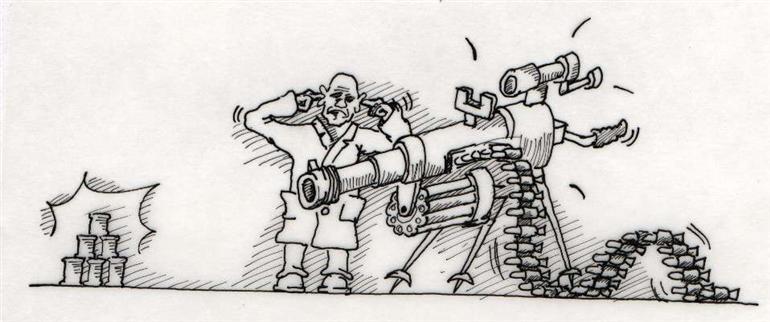
\includegraphics[width=0.8\textwidth]{lda/monte-carlo-simulation.jpg}
\caption{蒙特卡罗方法}
\end{figure}

统计模拟中有一个重要的问题就是给定一个概率分布$p(x)$,我们如何在计算机中生成它的样本。
一般而言均匀分布 $Uniform(0,1)$的样本是相对容易生成的。 通过线性同余发生器可以生成伪随机数,
我们用确定性算法生成$[0,1]$之间的伪随机数序列后,这些序列的各种统计指标和均匀分布 $Uniform(0,1)$
的理论计算结果非常接近。这样的伪随机序列就有比较好的统计性质,可以被当成真实的随机数使用。

\begin{figure}[htbp]
\centering
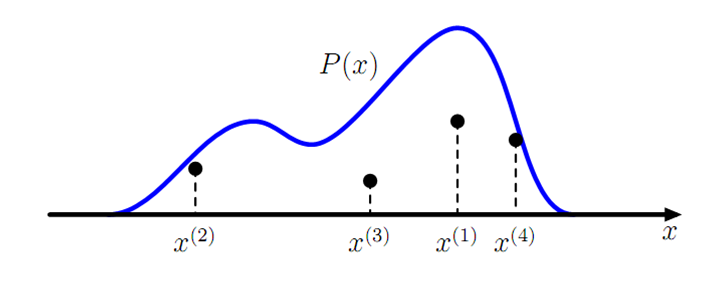
\includegraphics[width=0.8\textwidth]{lda/sampling.png}
\caption{生成一个概率分布的样本}
\end{figure}

而我们常见的概率分布,无论是连续的还是离散的分布,都可以基于$Uniform(0,1)$ 的样本生成。
例如正态分布可以通过著名的 Box-Muller 变换得到
\begin{theorem}[Box-Muller 变换]
如果随机变量 $U_1, U_2$ 独立且$U_1, U_2 \sim Uniform[0,1]$,则
\begin{align*}
Z_0 & = \sqrt{-2\ln U_1} cos(2\pi U_2) \\
Z_1 & = \sqrt{-2\ln U_1} sin(2\pi U_2)
\end{align*}
则, $Z_0,Z_1$ 独立且服从标准正态分布。
\end{theorem}

其它几个著名的连续分布,包括指数分布、Gamma 分布、t 分布、F 分布、Beta 分布、Dirichlet 分布
等等,也都可以通过类似的数学变换得到;离散的分布通过均匀分布更加容易生成。
更多的统计分布如何通过均匀分布的变换生成出来,大家可以参考统计计算的书,
其中 Sheldon M. Ross 的《统计模拟》是写得非常通俗易懂的一本。

不过我们并不是总是这么幸运的,当$p(x)$的形式很复杂,或者 $p(\mathbf{x})$ 是个高维的分布的时候,
样本的生成就可能很困难了。 譬如有如下的情况
\begin{enumerate}
\item  $\displaystyle p(x) = \frac{\tilde{p}(x)}{\int \tilde{p}(x) dx}$,
而 $\tilde{p}(x)$ 我们是可以计算的,但是底下的积分式无法显式计算。
\item $p(x,y)$ 是一个二维的分布函数,这个函数本身计算很困难,
但是条件分布 $p(x|y),p(y|x)$的计算相对简单;
如果 $p(\mathbf{x})$ 是高维的,这种情形就更加明显。
\end{enumerate}

此时就需要使用一些更加复杂的随机模拟的方法来生成样本。
而本节中将要重点介绍的 MCMC(Markov Chain Monte Carlo) 和
Gibbs Sampling算法就是最常用的一种,这两个方法在现代贝叶斯分析中被广泛使用。
要了解这两个算法,我们首先要对马氏链的平稳分布的性质有基本的认识。

\section{马氏链及其平稳分布}
马氏链的数学定义很简单
$$ P(X_{t+1}=x|X_t, X_{t-1}, \cdots) =P(X_{t+1}=x|X_t) $$
也就是状态转移的概率只依赖于前一个状态。

我们先来看马氏链的一个具体的例子。社会学家经常把人按其经济状况分成3类:
下层(lower-class)、中层(middle-class)、上层(upper-class),我们用1,2,3 分别
代表这三个阶层。社会学家们发现决定一个人的收入阶层的最重要的因素就是其父母
的收入阶层。如果一个人的收入属于下层类别,那么他的孩子属于下层收入的概率是
0.65, 属于中层收入的概率是 0.28, 属于上层收入的概率是 0.07。事实上,
从父代到子代,收入阶层的变化的转移概率如下

\begin{center}
\begin{tabular}{ccccc}
\hline
& & & 子代 &  \\
& State & 1 & 2 & 3 \\
\hline
     &1 & 0.65 & 0.28 & 0.07 \\
父代 & 2 & 0.15 & 0.67 & 0.18 \\
     & 3 & 0.12 & 0.36 & 0.52 \\
\end{tabular}
\end{center}

\begin{figure}[htbp]
\centering
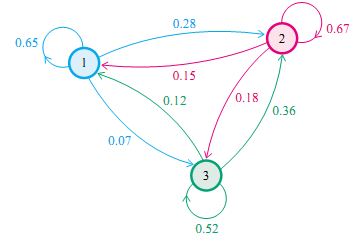
\includegraphics[width=0.6\textwidth]{lda/markov-transition.png}
\end{figure}

使用矩阵的表示方式,转移概率矩阵记为
$$P =
\begin{bmatrix}
0.65 & 0.28 & 0.07 \\
0.15 & 0.67 & 0.18 \\
0.12 & 0.36 & 0.52 \\
\end{bmatrix}
$$

假设当前这一代人处在下层、中层、上层的人的比例是概率分布向量 $\pi_0=[\pi_0(1), \pi_0(2), \pi_0(3)]$,
那么他们的子女的分布比例将是 $\pi_1=\pi_0P$, 他们的孙子代的分布比例将是 $\pi_2 = \pi_1P=\pi_0P^2$,
......, 第$n$代子孙的收入分布比例将是 $\pi_n = \pi_{n-1}P = \pi_0P^n$。

假设初始概率分布为$\pi_0 = [0.21,0.68,0.11] $,则我们可以计算前$n$代人的分布状况如下
\begin{center}
\begin{tabular}{clll}
第$n$代人 & 下层 & 中层 & 上层 \\
\hline
0 & 0.210 & 0.680 & 0.110 \\
1 & 0.252 & 0.554 & 0.194 \\
2 & 0.270 & 0.512 & 0.218 \\
3 & 0.278 & 0.497 & 0.225 \\
4 & 0.282 & 0.490 & 0.226 \\
5 & 0.285 & 0.489 & 0.225 \\
6 & 0.286 & 0.489 & 0.225 \\
7 & 0.286 & 0.489 & 0.225 \\
8 & 0.289 & 0.488 & 0.225 \\
9 & 0.286 & 0.489 & 0.225 \\
10 & 0.286 & 0.489 & 0.225 \\
$\cdots$  & $\cdots$  & $\cdots$  & $\cdots$  \\
\end{tabular}
\end{center}

我们发现从第7代人开始,这个分布就稳定不变了,这个是偶然的吗?
我们换一个初始概率分布$\pi_0 = [0.75,0.15,0.1]$ 试试看,继续计算前$n$代人的分布状况如下
\begin{center}
\begin{tabular}{clll}
第$n$代人 & 下层 & 中层 & 上层 \\
\hline
0 & 0.75 & 0.15 & 0.1 \\
1 & 0.522 & 0.347 & 0.132 \\
2 & 0.407 & 0.426 & 0.167 \\
3 & 0.349 & 0.459 & 0.192 \\
4 & 0.318 & 0.475 & 0.207 \\
5 & 0.303 & 0.482 & 0.215 \\
6 & 0.295 & 0.485 & 0.220 \\
7 & 0.291 & 0.487 & 0.222 \\
8 & 0.289 & 0.488 & 0.225 \\
9 & 0.286 & 0.489 & 0.225 \\
10 & 0.286 & 0.489 & 0.225 \\
$\cdots$  & $\cdots$  & $\cdots$  & $\cdots$  \\
\end{tabular}
\end{center}

我们发现,到第9代人的时候, 分布又收敛了。最为奇特的是,两次给定不同的初始概率分布,最终都收敛到
概率分布 $\pi=[0.286, 0.489, 0.225]$,也就是说收敛的行为和初始概率分布 $\pi_0$ 无关。
这说明这个收敛行为主要是由概率转移矩阵$P$决定的。我们计算一下 $P^n$
$$ P^{20} = P^{21} = \cdots = P^{100} = \cdots =
\begin{bmatrix}
0.286 & 0.489 & 0.225 \\
0.286 & 0.489 & 0.225 \\
0.286 & 0.489 & 0.225 \\
\end{bmatrix}
$$

我们发现,当 $n$ 足够大的时候,这个$P^n$矩阵的每一行都是稳定地收敛到$\pi=[0.286, 0.489, 0.225]$
这个概率分布。自然的,这个收敛现象并非是我们这个马氏链独有的,而是绝大多数马氏链的共同行为,
关于马氏链的收敛我们有如下漂亮的定理:

\begin{theorem} 如果一个非周期马氏链具有转移概率矩阵$P$,且它的任何两个状态是连通的,
那么 $\displaystyle \lim_{n\rightarrow\infty}P_{ij}^n$ 存在且与$i$无关,
记 $\displaystyle \lim_{n\rightarrow\infty}P_{ij}^n = \pi(j)$, 我们有
\begin{enumerate}
\item $ \displaystyle \lim_{n \rightarrow \infty} P^n =
\begin{bmatrix}
\pi(1) & \pi(2) & \cdots & \pi(j) & \cdots \\
\pi(1) & \pi(2) & \cdots & \pi(j) & \cdots \\
\cdots & \cdots & \cdots & \cdots & \cdots \\
\pi(1) & \pi(2) & \cdots & \pi(j) & \cdots \\
\cdots & \cdots & \cdots & \cdots & \cdots \\
\end{bmatrix} $
\item $ \displaystyle \pi(j) = \sum_{i=0}^{\infty}\pi(i)P_{ij} $
\item $\pi$ 是方程 $\pi P = \pi$ 的唯一非负解
\end{enumerate}
其中,
$$ \pi = [\pi(1), \pi(2), \cdots, \pi(j),\cdots ], \quad \sum_{i=0}^{\infty} \pi_i = 1  $$
$\pi$称为马氏链的平稳分布。
\end{theorem}


这个马氏链的收敛定理非常重要,\textbf{所有的 MCMC(Markov Chain Monte Carlo)
方法都是以这个定理作为理论基础的。}
定理的证明相对复杂,一般的随机过程课本中也不给证明,
所以我们就不用纠结它的证明了,直接用这个定理的结论就好了。我们对这个定理的内容做一些解释说明:
\begin{enumerate}
\item 该定理中马氏链的状态不要求有限,可以是有无穷多个的;
\item 定理中的“非周期“这个概念我们不打算解释了,因为我们遇到的绝大多数马氏链都是非周期的;
\item 两个状态$i,j$是连通并非指$i$ 可以直接一步转移到$j$($P_{ij} > 0$),而是指 $i$ 可以通过有限的$n$步
转移到达$j$($P_{ij}^n > 0$)。马氏链的任何两个状态是连通的含义是指存在一个$n$, 使得
矩阵$P^n$ 中的任何一个元素的数值都大于零。
\item 我们用 $X_i$ 表示在马氏链上跳转第$i$步后所处的状态,
如果 $\displaystyle \lim_{n\rightarrow\infty}P_{ij}^n = \pi(j)$ 存在,
很容易证明以上定理的第二个结论。由于
\begin{align*}
P(X_{n+1}=j) & = \sum_{i=0}^\infty P(X_n=i) P(X_{n+1}=j|X_n=i) \\
& = \sum_{i=0}^\infty P(X_n=i) P_{ij}
\end{align*}
上式两边取极限就得到 $ \displaystyle \pi(j) = \sum_{i=0}^{\infty}\pi(i)P_{ij}$
\end{enumerate}

从初始概率分布 $\pi_0$ 出发,我们在马氏链上做状态转移,记$X_i$的概率分布为$\pi_i$, 则有
\begin{align*}
X_0 & \sim \pi_0(x) \\
X_i & \sim \pi_i(x),  \quad\quad \pi_i(x) = \pi_{i-1}(x)P = \pi_0(x)P^n
\end{align*}
由马氏链收敛的定理, 概率分布$\pi_i(x)$将收敛到平稳分布 $\pi(x)$。假设到第$n$步
的时候马氏链收敛,则有
\begin{align*}
X_0 & \sim \pi_0(x) \\
X_1 & \sim \pi_1(x) \\
& \cdots \\
X_n & \sim \pi_n(x)=\pi(x) \\
X_{n+1} & \sim \pi(x) \\
X_{n+2}& \sim \pi(x) \\
& \cdots
\end{align*}
所以 $X_n,X_{n+1},X_{n+2},\cdots \sim \pi(x)$ 都是同分布的随机变量,当然他们并不独立。
如果我们从一个具体的初始状态 $x_0$ 开始,沿着马氏链按照概率转移矩阵做跳转,
那么我们得到一个转移序列 $x_0, x_1, x_2, \cdots x_n, x_{n+1}\cdots,$
由于马氏链的收敛行为, $x_n, x_{n+1},\cdots$ 都将是平稳分布 $\pi(x)$ 的样本。

\section{Markov Chain Monte Carlo}
对于给定的概率分布$p(x)$,我们希望能有便捷的方式生成它对应的样本。
由于马氏链能收敛到平稳分布, 于是一个很的漂亮想法是:如果我们能构造一个转移矩阵为$P$的马氏链,
使得该马氏链的平稳分布恰好是$p(x)$,
那么我们从任何一个初始状态$x_0$出发沿着马氏链转移, 得到一个转移序列
$x_0, x_1, x_2, \cdots x_n, x_{n+1}\cdots,$, 如果马氏链在第$n$步已经收敛了,于是我们就得到了
$\pi(x)$ 的样本$x_n, x_{n+1}\cdots$。

这个绝妙的想法在1953年被 Metropolis想到了,为了研究粒子系统的平稳性质,
Metropolis 考虑了物理学中常见的波尔兹曼分布的采样问题,首次提出了基于马氏链的蒙特卡罗方法,
即Metropolis算法,并在最早的计算机上编程实现。Metropolis 算法是首个普适的采样方法,
并启发了一系列 MCMC方法,所以人们把它视为随机模拟技术腾飞的起点。
Metropolis的这篇论文被收录在《统计学中的重大突破》中,
Metropolis算法也被遴选为二十世纪的十个最重要的算法之一。

我们接下来介绍的MCMC 算法是 Metropolis 算法的一个改进变种,即常用的 Metropolis-Hastings 算法。
由上一节的例子和定理我们看到了,马氏链的收敛性质主要由转移矩阵$P$ 决定,
所以基于马氏链做采样的关键问题是如何构造转移矩阵$P$,使得平稳分布恰好是我们要的分布$p(x)$。
如何能做到这一点呢?我们主要使用如下的定理。

\begin{theorem}[细致平稳条件]
如果非周期马氏链的转移矩阵$P$和分布$\pi(x)$ 满足
\begin{equation}
\pi(i)P_{ij} = \pi(j)P_{ji} \quad\quad \text{for all} \quad i,j
\end{equation}
则 $\pi(x)$ 是马氏链的平稳分布,上式被称为细致平稳条件(detailed balance condition)。
\end{theorem}

其实这个定理是显而易见的,因为细致平稳条件的物理含义就是对于任何两个状态$i,j$,
从 $i$ 转移出去到$j$ 而丢失的概率质量,恰好会被从 $j$ 转移回$i$ 的概率质量补充回来,
所以状态$i$上的概率质量$\pi(i)$是稳定的,从而$\pi(x)$是马氏链的平稳分布。
数学上的证明也很简单,由细致平稳条件可得
\begin{align*}
& \sum_{i=1}^\infty \pi(i)P_{ij} = \sum_{i=1}^\infty \pi(j)P_{ji}
= \pi(j) \sum_{i=1}^\infty P_{ji} = \pi(j) \\
& \Rightarrow \pi P = \pi
\end{align*}
由于$\pi$ 是方程 $\pi P = \pi$的解,所以$\pi$是平稳分布。


假设我们已经有一个转移矩阵为$Q$马氏链($q(i,j)$表示从状态 $i$转移到状态$j$的概率,
也可以写为 $q(j|i)$或者$q(i\rightarrow j)$),
显然,通常情况下
$$ p(i) q(i,j) \neq p(j) q(j,i) $$
也就是细致平稳条件不成立,所以 $p(x)$ 不太可能是这个马氏链的平稳分布。
我们可否对马氏链做一个改造,使得细致平稳条件成立呢?譬如,我们引入一个 $\alpha(i,j)$,
我们希望
\begin{equation}
\label{choose-alpha}
 p(i) q(i,j)\alpha(i,j) = p(j) q(j,i)\alpha(j,i)
\end{equation}
取什么样的 $\alpha(i,j)$ 以上等式能成立呢?最简单的,按照对称性,我们可以取
$$ \alpha(i,j)= p(j) q(j,i), \quad \alpha(j,i) = p(i) q(i,j)$$
于是\eqref{choose-alpha}式就成立了。所以有
\begin{equation}
\label{detailed-balance}
p(i) \underbrace{q(i,j)\alpha(i,j)}_{Q'(i,j)}
= p(j) \underbrace{q(j,i)\alpha(j,i)}_{Q'(j,i)}
\end{equation}
于是我们把原来具有转移矩阵$Q$的一个很普通的马氏链,改造为了具有转移矩阵$Q'$的马氏链,而
$Q'$恰好满足细致平稳条件,由此马氏链$Q'$的平稳分布就是$p(x)$!

在改造 $Q$ 的过程中引入的 $\alpha(i,j)$称为接受率,物理意义可以理解为在原来的马氏链上,
从状态 $i$ 以$q(i,j)$ 的概率转跳转到状态$j$ 的时候,我们以$\alpha(i,j)$的概率接受这个转移,于
是得到新的马氏链$Q'$的转移概率为$q(i,j)\alpha(i,j)$。

\begin{figure}[htbp]
\centering
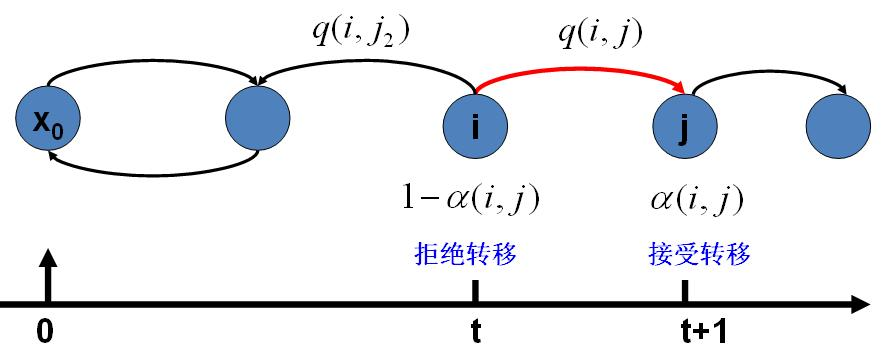
\includegraphics[width=0.9\textwidth]{lda/mcmc-transition.jpg}
\caption{马氏链转移和接受概率}
\end{figure}

假设我们已经有一个转移矩阵Q(对应元素为$q(i,j)$), 把以上的过程整理一下,
我们就得到了如下的用于采样概率分布$p(x)$的算法。
\begin{algorithm}[h]
\caption{MCMC 采样算法}
\begin{algorithmic}[1]
\STATE 初始化马氏链初始状态 $X_0 = x_0$
\STATE 对 $t=0,1,2,\cdots$, 循环以下过程进行采样
\begin{itemize}
\item 第$t$个时刻马氏链状态为 $X_t=x_t$, 采样 $y \sim q(x|x_t)$
\item 从均匀分布采样 $u \sim Uniform[0,1]$
\item 如果 $u < \alpha(x_t,y) = p(y)q(x_t|y)$ 则接受转移$x_t\rightarrow y$, 即$X_{t+1} = y$
\item 否则不接受转移, 即$X_{t+1} = x_t$
\end{itemize}
\end{algorithmic}
\end{algorithm}

上述过程中 $p(x),q(x|y)$ 说的都是离散的情形,事实上即便这两个分布是连续的,以上算法仍然是有效,
于是就得到更一般的连续概率分布 $p(x)$的采样算法,而 $q(x|y)$ 就是任意一个连续二元概率分布对应的条件分布。

以上的 MCMC 采样算法已经能很漂亮的工作了,不过它有一个小的问题:马氏链$Q$在转移的过程中的接受率 $\alpha(i,j)$
可能偏小,这样采样过程中马氏链容易原地踏步,拒绝大量的跳转,这使得马氏链遍历所有的状态空间要花费太长的时间,
收敛到平稳分布$p(x)$的速度太慢。有没有办法提升一些接受率呢?

假设 $\alpha(i,j)=0.1, \alpha(j,i)=0.2$, 此时满足细致平稳条件,于是
$$ p(i)q(i,j)\times 0.1 = p(j)q(j,i) \times 0.2 $$
上式两边扩大5倍,我们改写为
$$ p(i)q(i,j) \times 0.5 = p(j)q(j,i) \times 1 $$
看,我们提高了接受率,而细致平稳条件并没有打破!这启发我们可以把细致平稳条件
\eqref{detailed-balance}式中的$\alpha(i,j),\alpha(j,i)$ 同比例放大,
使得两数中最大的一个放大到1,这样我们就提高了采样中的跳转接受率。
所以我们可以取
$$ \alpha(i,j) = \min\left\{\frac{p(j)q(j,i)}{p(i)q(i,j)},1\right\} $$
于是,经过对上述MCMC 采样算法中接受率的微小改造,我们就得到了如下教科书中最常见的 Metropolis-Hastings 算法。
\begin{algorithm}[htb]
\caption{Metropolis-Hastings 采样算法}
\begin{algorithmic}[1]
\STATE 初始化马氏链初始状态 $X_0 = x_0$
\STATE 对 $t=0,1,2,\cdots$, 循环以下过程进行采样
\begin{itemize}
\item 第$t$个时刻马氏链状态为 $X_t=x_t$, 采样 $y \sim q(x|x_t)$
\item 从均匀分布采样 $u \sim Uniform[0,1]$
\item 如果 $u < \alpha(x_t,y) = \min\left\{\frac{p(y)q(x_t|y)}{p(x_t)p(y|x_t)},1\right\}$
      则接受转移$x_t\rightarrow y$, 即 $X_{t+1} = y$
\item 否则不接受转移, 即 $X_{t+1} = x_t$
\end{itemize}
\end{algorithmic}
\end{algorithm}

对于分布 $p(x)$,我们构造转移矩阵 $Q'$ 使其满足细致平稳条件
$$ p(x) Q'(x\rightarrow y) = p(y) Q'(y\rightarrow x) $$
此处 $x$ 并不要求是一维的,对于高维空间的 $p(\mathbf{x})$,如果满足细致平稳条件
$$ p(\mathbf{x}) Q'(\mathbf{x}\rightarrow \mathbf{y})
= p(\mathbf{y}) Q'(\mathbf{y}\rightarrow \mathbf{x}) $$
那么以上的 Metropolis-Hastings 算法一样有效。

\section{Gibbs Sampling}
对于高维的情形,由于接受率 $\alpha$的存在(通常 $\alpha < 1$), 以上 Metropolis-Hastings 算法的效率不够高。
能否找到一个转移矩阵Q使得接受率 $\alpha=1$ 呢?
我们先看看二维的情形,假设有一个概率分布 $p(x,y)$, 考察$x$坐标相同的
两个点$A(x_1,y_1), B(x_1,y_2)$,我们发现
\begin{align*}
p(x_1,y_1)p(y_2|x_1) = p(x_1)p(y_1|x_1)p(y_2|x_1) \\
p(x_1,y_2)p(y_1|x_1) = p(x_1)p(y_2|x_1)p(y_1|x_1)
\end{align*}
所以得到
\begin{equation}
\label{gibbs-detailed-balance}
 p(x_1,y_1)p(y_2|x_1) =  p(x_1,y_2)p(y_1|x_1)
\end{equation}
即
$$ p(A)p(y_2|x_1) =  p(B)p(y_1|x_1) $$
基于以上等式,我们发现,在 $x=x_1$ 这条平行于 $y$轴的直线上,
如果使用条件分布 $p(y|x_1)$做为任何两个点之间的转移概率,
那么任何两个点之间的转移满足细致平稳条件。同样的,如果我们在 $y=y_1$ 这条直线上任意取两个点
$A(x_1,y_1), C(x_2,y_1)$,也有如下等式
$$ p(A)p(x_2|y_1) =  p(C)p(x_1|y_1). $$

\begin{figure}[h]
\centering
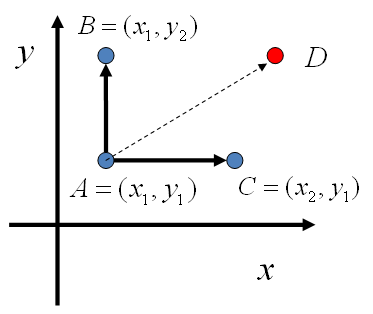
\includegraphics[width=0.5\textwidth]{lda/gibbs-transition.png}
\caption{平面上马氏链转移矩阵的构造}
\end{figure}

于是我们可以如下构造平面上任意两点之间的转移概率矩阵Q
\begin{align*}
Q(A\rightarrow B) & = p(y_B|x_1) & \text{如果} \quad x_A=x_B=x_1 & \\
Q(A\rightarrow C) & = p(x_C|y_1) & \text{如果} \quad y_A=y_C=y_1 & \\
Q(A\rightarrow D) & = 0          & \text{其它} &
\end{align*}


有了如上的转移矩阵 Q, 我们很容易验证对平面上任意两点 $X,Y$, 满足细致平稳条件
$$ p(X)Q(X\rightarrow Y) = p(Y) Q(Y\rightarrow X) $$
于是这个二维空间上的马氏链将收敛到平稳分布 $p(x,y)$。
而这个算法就称为 Gibbs Sampling 算法,由物理学家 Gibbs 首先给出的。

\begin{algorithm}[htb]
\caption{二维Gibbs Sampling 算法}
\begin{algorithmic}[1]
\STATE 随机初始化 $X_0 = x_0,Y_0=y_0$
\STATE 对 $t=0,1,2,\cdots$ 循环采样
\begin{enumerate}
\item  $y_{t+1} \sim p(y|x_{t})$
\item  $x_{t+1} \sim p(x|y_{t+1})$
\end{enumerate}
\end{algorithmic}
\end{algorithm}
\begin{figure}[htbp]
\centering
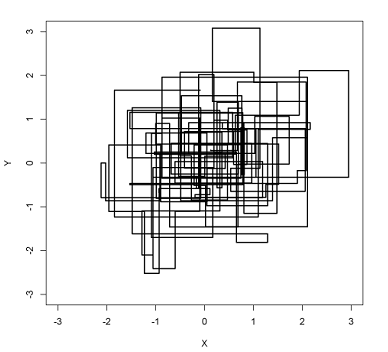
\includegraphics[width=0.6\textwidth]{lda/two-stage-gibbs.png}
\caption{二维Gibbs Sampling 算法中的马氏链转移}
\end{figure}

以上采样过程中,如图所示,马氏链的转移只是轮换的沿着坐标轴 $x$轴和$y$轴做转移,于是
得到样本 $(x_0,y_0), (x_0,y_1), (x_1,y_1), (x_1,y_2),(x_2,y_2), \cdots $
马氏链收敛后,最终得到的样本就是 $p(x,y)$ 的样本,而收敛之前的阶段称为 burn-in period。
额外说明一下,我们看到教科书上的 Gibbs Sampling 算法大都是坐标轴轮换采样的,
但是这其实是不强制要求的。最一般的情形可以是,在$t$时刻,
可以在$x$轴和$y$轴之间随机的选一个坐标轴,然后按条件概率做转移,
马氏链也是一样收敛的。轮换两个坐标轴只是一种方便的形式。

以上的过程我们很容易推广到高维的情形,对于\eqref{gibbs-detailed-balance}式,
如果$x_1$ 变为多维情形$\mathbf{x_1}$,可以看出推导过程不变,所以细致平稳条件同样是成立的
\begin{equation}
\label{gibbs-detailed-balance-n-dimen}
p(\mathbf{x_1},y_1)p(y_2|\mathbf{x_1}) =  p(\mathbf{x_1},y_2)p(y_1|\mathbf{x_1})
\end{equation}
此时转移矩阵 Q 由条件分布 $p(y|\mathbf{x_1})$ 定义。
上式只是说明了一根坐标轴的情形,和二维情形类似,很容易验证对所有坐标轴都有类似的结论。
所以$n$维空间中对于概率分布 $p(x_1,x_2,\cdots, x_n)$ 可以如下定义转移矩阵

\begin{enumerate}
\item 如果当前状态为$(x_1,x_2,\cdots, x_n)$,马氏链转移的过程中,只能沿着坐标轴做转移。
沿着 $x_i$ 这根坐标轴做转移的时候,转移概率由条件概率
 $p(x_i|x_1, \cdots, x_{i-1}, x_{i+1}, \cdots, x_n)$ 定义;
\item 其它无法沿着单根坐标轴进行的跳转,转移概率都设置为 0。
\end{enumerate}

于是我们可以把Gibbs Smapling 算法从采样二维的 $p(x,y)$ 推广到采样$n$ 维的 $p(x_1,x_2,\cdots, x_n)$
\begin{algorithm}[htb]
\caption{n维Gibbs Sampling 算法}
\begin{algorithmic}[1]
\STATE 随机初始化 $\{x_i : i =1, \cdots, n\}$
\STATE 对 $t=0,1,2,\cdots$ 循环采样
\begin{enumerate}
\item  $x_1^{(t+1)} \sim p(x_1|x_2^{(t)}, x_3^{(t)}, \cdots, x_n^{(t)})$
\item  $x_2^{(t+1)} \sim p(x_2|x_1^{(t+1)}, x_3^{(t)}, \cdots, x_n^{(t)})$
\item  $\cdots$
\item  $x_j^{(t+1)} \sim p(x_j|x_1^{(t+1)}, \cdots, x_{j-1}^{(t+1)}, x_{j+1}^{(t)}, \cdots, x_n^{(t)})$
\item  $\cdots$
\item  $x_n^{(t+1)} \sim p(x_n|x_1^{(t+1)}, x_2^t, \cdots, x_{n-1}^{(t+1)})$
\end{enumerate}
\end{algorithmic}
\end{algorithm}

以上算法收敛后,得到的就是概率分布$p(x_1,x_2,\cdots, x_n)$的样本,当然这些样本并不独立,
但是我们此处要求的是采样得到的样本符合给定的概率分布,并不要求独立。同样的,在以上算法中,
坐标轴轮换采样不是必须的,可以在坐标轴轮换中引入随机性,这时候转移矩阵 $Q$ 中任何两个点
的转移概率中就会包含坐标轴选择的概率,而在通常的 Gibbs Sampling 算法中,坐标轴轮换是一个确定
性的过程,也就是在给定时刻$t$,在一根固定的坐标轴上转移的概率是1。


